
%(BEGIN_QUESTION)
% Copyright 2010, Tony R. Kuphaldt, released under the Creative Commons Attribution License (v 1.0)
% This means you may do almost anything with this work of mine, so long as you give me proper credit

A technician has wired a proximity switch to a relay, such that one LED lamp is supposed to come on when nothing is near the switch, and the other lamp is supposed to come on when the switch detects the presence of a metal object:

$$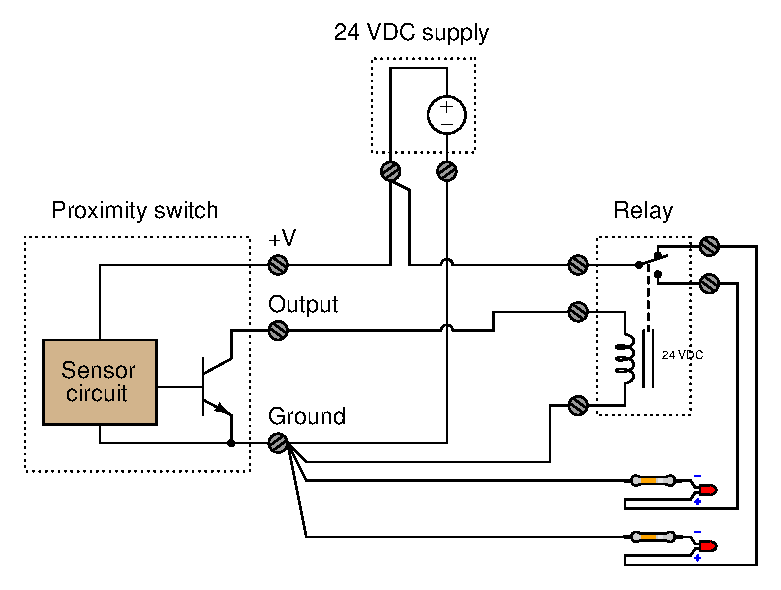
\includegraphics[width=15.5cm]{i03759x01.eps}$$

However, there is a problem in the wiring of this circuit.  First, identify what this circuit will {\it actually} do.  Next, identify the wiring problem and propose a correction so that the circuit will function as it was intended.

\vskip 20pt \vbox{\hrule \hbox{\strut \vrule{} {\bf Suggestions for Socratic discussion} \vrule} \hrule}

\begin{itemize}
\item{} Is this a {\it sinking} or a {\it sourcing} proximity switch?  How can we tell?
\item{} This is a very common wiring mistake seen in student work.  Explain why many people are tempted to make this mistake, and how it may be avoided by thinking more carefully about the circuit's function.
\end{itemize}

\underbar{file i03759}
%(END_QUESTION)





%(BEGIN_ANSWER)

The way this circuit is presently wired, the lower LED will always be on regardless of proximity switch status.

%(END_ANSWER)





%(BEGIN_NOTES)

The problem here is that both the proximity switch and the relay are connected to {\it sink} current.  One of these two needs to sink while the other needs to source, in order for the circuit to work as it should.  Thus, there are multiple correct solutions to this problem.

\vskip 10pt

Another (minor) problem is that the technician has placed {\it four} wires under the same terminal (on the prox switch), which is a wiring {\it faux pax}.

\vskip 10pt

Here is a suggested re-wiring of the circuit:

$$\includegraphics[width=15.5cm]{i03759x04.eps}$$






\vskip 20pt \vbox{\hrule \hbox{\strut \vrule{} {\bf Virtual Troubleshooting} \vrule} \hrule}

This question is a good candidate for a ``Virtual Troubleshooting'' exercise.  Presenting the diagram to students, you first imagine in your own mind a particular fault in the system.  Then, you present one or more symptoms of that fault (something noticeable by an operator or other user of the system).  Students then propose various diagnostic tests to perform on this system to identify the nature and location of the fault, as though they were technicians trying to troubleshoot the problem.  Your job is to tell them what the result(s) would be for each of the proposed diagnostic tests, documenting those results where all the students can see.

During and after the exercise, it is good to ask students follow-up questions such as:

\begin{itemize}
\item{} What does the result of the last diagnostic test tell you about the fault?
\item{} Suppose the results of the last diagnostic test were different.  What then would that result tell you about the fault?
\item{} Is the last diagnostic test the best one we could do?
\item{} What would be the ideal order of tests, to diagnose the problem in as few steps as possible?
\end{itemize}

\vfil \eject

\noindent
{\bf Summary Quiz:}

Identify whether the proximity switch shown in this schematic diagram is a {\it sourcing} type or a {\it sinking} type:

$$\includegraphics[width=15.5cm]{i03759x02.eps}$$


\vfil \eject

\noindent
{\bf Summary Quiz:}

Identify whether the proximity switch shown in this schematic diagram is a {\it sourcing} type or a {\it sinking} type:

$$\includegraphics[width=15.5cm]{i03759x03.eps}$$


%INDEX% Switch, proximity: sourcing versus sinking output

%(END_NOTES)

